\chapter{Metodología e implementación}
\label{cap:metodologia}

El Capítulo~\ref{cap:propuesta} describió \textit{qué} se propone construir y con qué diseño. Este capítulo describe \textit{cómo} se ha llevado esa propuesta a la práctica: la metodología de trabajo seguida durante el desarrollo, el entorno y las herramientas técnicas empleadas, el esquema completo de la base de datos espacial resultante, y la organización del código fuente del proyecto, tanto de los procesos ETL como del prototipo de visor web.

% -----------------------------------------------------------------------
% 4.1 METODOLOGÍA DE DESARROLLO
% -----------------------------------------------------------------------
\section{Metodología de desarrollo}
\label{sec:metodologia_desarrollo}

El desarrollo se ha organizado siguiendo un enfoque \textbf{incremental por fuente de datos}: en lugar de diseñar de antemano el esquema completo de la base de datos y cargar todas las fuentes a la vez, cada fuente de riesgo se ha incorporado como un incremento independiente, verificado antes de pasar al siguiente. Esto se refleja directamente en la numeración de los scripts de \texttt{scripts/}, que documenta el orden real en que se desarrolló el sistema:

\begin{enumerate}
    \item \texttt{01\_download\_osm.py} — descarga de la red viaria peatonal con \texttt{osmnx}.
    \item \texttt{02\_load\_osm\_to\_db.py} — carga de nodos y aristas en PostgreSQL/PostGIS.
    \item \texttt{03\_load\_farolas.py} — carga de la iluminación pública y cálculo del indicador por tramo.
    \item \texttt{04\_load\_accidentes.py} — carga de accidentes y cálculo de los indicadores de siniestralidad y atropellos.
    \item \texttt{05\_load\_vulnerabilidad.py} — carga del Índice Iguala Madrid por distrito.
    \item \texttt{06\_load\_distritos.py} — carga de los polígonos de distrito y join espacial tramo-distrito.
    \item \texttt{07\_calcular\_indice\_seguridad.py} — combinación de los indicadores anteriores en el índice de peligrosidad y el coste seguro.
    \item \texttt{08\_calcular\_ruta.py} y \texttt{rutas.py} — algoritmo de enrutamiento, primero como script de línea de comandos y después como módulo reutilizable.
\end{enumerate}

Esta organización tiene una consecuencia directa sobre el esquema de la base de datos: la tabla \texttt{edges} no nace con todas sus columnas, sino que se \textbf{amplía progresivamente} a medida que cada nueva fuente de datos aporta un indicador adicional, mediante sentencias \texttt{ALTER TABLE ADD COLUMN IF NOT EXISTS} en el script SQL de cada fuente (Sección~\ref{sec:esquema_bd}).

Cada script sigue además el mismo patrón de \textbf{idempotencia}: al inicio comprueba si los datos correspondientes ya están cargados (mediante un \texttt{SELECT count(*)} sobre la tabla destino) y, si es así, no hace nada, salvo que una variable \texttt{OVERWRITE} se ponga explícitamente a \texttt{True}. Esto permite ejecutar el pipeline completo repetidamente durante el desarrollo —por ejemplo, tras corregir un error en un script posterior— sin volver a descargar o recalcular lo ya procesado, y sin arriesgarse a duplicar filas por una ejecución accidental.

Tras cada incremento se ha aplicado una \textbf{verificación de control} mediante consultas SQL directas: recuento de filas cargadas, rango de valores de los indicadores calculados, y proporción de tramos afectados (por ejemplo, comprobar que el 100\,\% de los tramos quedan asignados a un distrito tras el \textit{join} espacial, o que la distribución del índice de peligrosidad resultante cae dentro de $[0, 1]$). Esta práctica ha permitido detectar durante el desarrollo, entre otros, el problema de las densidades desproporcionadas en tramos de longitud casi nula que motivó el recorte al percentil 99 descrito en la Sección~\ref{subsec:transformacion}.

Por último, el proyecto se ha versionado con \textbf{Git} desde su inicio, con un commit por hito funcional (una fuente de datos cargada, el índice de seguridad calculado, el algoritmo de enrutamiento funcionando, cada mejora del visor web), lo que ha permitido reconstruir con precisión, ya en fase de redacción de esta memoria, el orden real en que se tomaron las decisiones de diseño.

% -----------------------------------------------------------------------
% 4.2 ENTORNO Y HERRAMIENTAS DE DESARROLLO
% -----------------------------------------------------------------------
\section{Entorno y herramientas de desarrollo}
\label{sec:entorno_herramientas}

La Tabla~\ref{tab:stack} resume las principales tecnologías y versiones empleadas en el desarrollo.

\begin{table}[h]
\centering
\begin{tabular}{ll}
\hline
\textbf{Componente} & \textbf{Versión} \\
\hline
PostgreSQL & 16 \\
PostGIS & 3.4 \\
pgRouting & 3.6 \\
Python & 3.12 \\
osmnx & 2.1.0 \\
GeoPandas & 1.1.3 \\
Pandas & 3.0.3 \\
SQLAlchemy & 2.0.43 \\
GeoAlchemy2 & 0.18.0 \\
psycopg2-binary & 2.9.10 \\
Flask & 3.1.3 \\
Leaflet & 1.9.4 \\
\hline
\end{tabular}
\caption{Principales componentes del \textit{stack} tecnológico y versión utilizada.}
\label{tab:stack}
\end{table}

El entorno de desarrollo Python se gestiona mediante un entorno virtual (\texttt{venv}) aislado del sistema, con las dependencias fijadas por versión exacta en \texttt{requirements.txt} para garantizar la reproducibilidad del entorno. Las credenciales de acceso a la base de datos (usuario, contraseña, host, puerto y nombre de la base de datos \texttt{safe\_maps}) se externalizan en un fichero \texttt{.env}, cargado en tiempo de ejecución mediante \texttt{python-dotenv} y excluido explícitamente del control de versiones, de forma que ningún secreto queda expuesto en el repositorio público del proyecto.

% -----------------------------------------------------------------------
% 4.3 ESQUEMA DE LA BASE DE DATOS
% -----------------------------------------------------------------------
\section{Esquema de la base de datos espacial}
\label{sec:esquema_bd}

La base de datos \texttt{safe\_maps} está compuesta por seis tablas, cada una introducida por el script ETL de su fuente de datos correspondiente (Sección~\ref{sec:metodologia_desarrollo}). La Tabla~\ref{tab:tablas_bd} resume su propósito y volumen tras la carga completa.

\begin{table}[h]
\centering
\small
\begin{tabular}{lp{6.5cm}r}
\hline
\textbf{Tabla} & \textbf{Contenido} & \textbf{Filas} \\
\hline
\texttt{nodes} & Nodos de la red viaria (intersecciones) & 174\,394 \\
\texttt{edges} & Tramos de calle, con los indicadores de riesgo y el coste de enrutamiento & 524\,292 \\
\texttt{farolas} & Unidades luminosas del alumbrado público & 233\,309 \\
\texttt{accidentes} & Accidentes de tráfico 2023-2025, uno por expediente & 63\,042 \\
\texttt{vulnerabilidad\_distritos} & Índice Iguala por distrito (año 2024) & 21 \\
\texttt{distritos} & Polígonos administrativos de los distritos & 21 \\
\hline
\end{tabular}
\caption{Tablas de la base de datos \texttt{safe\_maps} y su volumen tras la carga completa.}
\label{tab:tablas_bd}
\end{table}

\texttt{nodes} y \texttt{edges} constituyen el grafo viario propiamente dicho (Sección~\ref{sec:modelado_red}) y son las únicas tablas con la estructura de nodos/aristas que exige pgRouting. Las cuatro tablas restantes son fuentes de datos auxiliares que \textbf{no participan directamente en \texttt{pgr\_dijkstra}}: su función es aportar, mediante uniones espaciales o por clave de distrito, los valores con los que se rellenan las columnas de indicadores de \texttt{edges}. La Tabla~\ref{tab:columnas_edges} detalla las columnas de \texttt{edges}, agrupadas según el script que las incorpora.

\begin{table}[h]
\centering
\small
\begin{tabular}{p{4cm}p{5.2cm}p{3cm}}
\hline
\textbf{Columnas} & \textbf{Descripción} & \textbf{Origen} \\
\hline
\texttt{\small id, u, v, key, source, target, highway, name, oneway, length, cost, reverse\_cost, geom} & Identificadores del tramo y de sus nodos extremo, atributos de OSM y geometría (\texttt{cost}/\texttt{reverse\_cost} = \texttt{length}) & \texttt{\small 02\_load\_osm\_to\_db} \\
\hline
\texttt{num\_farolas, farolas\_100m} & Nº de farolas en el buffer y su densidad & \texttt{\small 03\_load\_farolas} \\
\hline
\texttt{\small num\_accidentes, accidentes\_100m, num\_atropellos} & Nº de accidentes y de atropellos en el buffer, y densidad de accidentes & \texttt{\small 04\_load\_accidentes} \\
\hline
\texttt{cod\_distrito} & Distrito asignado por \textit{join} espacial & \texttt{\small 06\_load\_distritos} \\
\hline
\texttt{\small indice\_peligrosidad, cost\_seguro, reverse\_cost\_seguro} & Índice de peligrosidad (Ecuación~\ref{eq:coste}) y coste de enrutamiento seguro & \texttt{\small 07\_calcular\_}\newline\texttt{\small indice\_seguridad} \\
\hline
\end{tabular}
\caption{Columnas de \texttt{edges}, agrupadas por el script que las incorpora.}
\label{tab:columnas_edges}
\end{table}

\begin{sloppypar}
Todas las tablas con columna de geometría (\texttt{nodes}, \texttt{edges}, \texttt{farolas}, \texttt{accidentes}, \texttt{distritos}) tienen un índice espacial \texttt{GIST} sobre dicha columna, imprescindible para que las consultas de proximidad (\texttt{ST\_DWithin}, \texttt{ST\_Within}, el operador de vecino más cercano \texttt{<->}) utilizadas en el proceso ETL y en el enrutamiento se resuelvan en tiempo razonable sobre una red de más de medio millón de tramos. \texttt{edges} tiene además índices B-tree sobre \texttt{source} y \texttt{target}, requeridos por pgRouting para resolver eficientemente los recorridos del grafo. El código SQL completo de creación de cada tabla se encuentra en \texttt{sql/01\_schema.sql} a \texttt{sql/06\_indice\_seguridad.sql}.
\end{sloppypar}

% -----------------------------------------------------------------------
% 4.4 ORGANIZACIÓN DEL CÓDIGO
% -----------------------------------------------------------------------
\section{Organización del código fuente}
\label{sec:organizacion_codigo}

El repositorio del proyecto se organiza en los siguientes directorios principales:

\begin{itemize}
    \item \texttt{scripts/} — los ocho scripts ETL y de cálculo descritos en la Sección~\ref{sec:metodologia_desarrollo}, más el módulo \texttt{rutas.py} y los scripts \texttt{09\_evaluacion.py} y \texttt{10\_mapa\_peligrosidad.py}, usados respectivamente para la evaluación comparativa del Capítulo~\ref{cap:pruebas} y para generar la Figura~\ref{fig:mapa_peligrosidad}.
    \item \texttt{sql/} — un fichero de esquema SQL por cada fuente de datos, ejecutado por su script correspondiente al inicio de cada ejecución.
    \item \texttt{data/raw/} y \texttt{data/processed/} — datos originales descargados y datos derivados (como las rutas de ejemplo exportadas a GeoJSON), excluidos del control de versiones por su tamaño.
    \item \texttt{web/} — el prototipo de visor cartográfico (Sección~\ref{sec:backend_visor}).
    \item \texttt{docs/} — la presente memoria, en \LaTeX.
\end{itemize}

\begin{sloppypar}
Todos los scripts de \texttt{scripts/} comparten una misma estructura: resuelven la ruta base del proyecto de forma independiente del directorio de trabajo actual (\texttt{Path(\_\_file\_\_).parent.parent}), cargan las credenciales desde \texttt{.env}, ejecutan el esquema SQL de su fuente de datos, y aplican el patrón de idempotencia descrito en la Sección~\ref{sec:metodologia_desarrollo}. Esta redundancia deliberada entre scripts —en lugar de extraer, por ejemplo, la creación de la conexión a una función compartida— responde a que cada script está pensado para poder leerse y ejecutarse de forma autónoma, sin necesidad de entender el resto del pipeline; el único código realmente compartido es \texttt{rutas.py}, que expone la función \texttt{calcular\_ruta()} usada tanto por el script de línea de comandos \texttt{08\_calcular\_ruta.py} como por el backend del visor web, evitando así duplicar la lógica de enrutamiento —la única parte del sistema con dos consumidores distintos.
\end{sloppypar}

% -----------------------------------------------------------------------
% 4.5 IMPLEMENTACIÓN DEL BACKEND DEL VISOR
% -----------------------------------------------------------------------
\section{Implementación del backend del visor}
\label{sec:backend_visor}

El backend del prototipo se implementa como una aplicación \textbf{Flask} de un único fichero (\texttt{web/app.py}), que expone cuatro rutas HTTP:

\begin{itemize}
    \item \texttt{GET /} — sirve la página HTML del visor.
    \item \texttt{GET /api/ruta} — recibe las coordenadas de origen y destino como parámetros de consulta e invoca \texttt{calcular\_ruta()} (Sección~\ref{sec:enrutamiento}) una vez por cada criterio (\texttt{rapida} y \texttt{segura}), en paralelo mediante un \texttt{ThreadPoolExecutor} —cada hilo con su propia conexión a la base de datos, ya que los objetos \texttt{Connection} de SQLAlchemy no son seguros para compartir entre hilos—, y devuelve ambos resultados en un único objeto JSON.
    \item \texttt{GET /api/geocode} — recibe un texto de búsqueda y consulta en paralelo (mediante un \texttt{ThreadPoolExecutor}) dos servicios de geocodificación: \textbf{CartoCiudad}, el geocodificador oficial del Instituto Geográfico Nacional basado en el Catastro, y \textbf{Nominatim}, el geocodificador de OpenStreetMap. Ambos son complementarios: CartoCiudad resuelve con precisión el número de portal de cualquier dirección de Madrid —algo que Nominatim solo consigue cuando existe en OSM un punto de interés etiquetado con ese número exacto—, mientras que Nominatim es quien indexa nombres de establecimientos y lugares (comercios, museos, monumentos) que no tienen entrada en el Catastro. Los resultados de ambos se combinan, se eliminan duplicados —tanto por proximidad de coordenadas como por coincidencia del texto mostrado— y se devuelven ya divididos en una línea principal y una línea secundaria de contexto (barrio, distrito o municipio).
    \item \texttt{GET /api/geocode/inverso} — recibe unas coordenadas y devuelve la dirección más cercana vía Nominatim, usada al hacer clic directamente sobre el mapa.
\end{itemize}

Que el backend actúe como intermediario de estos servicios, en lugar de que el cliente los consulte directamente, tiene varios motivos: permite fijar desde el servidor una cabecera \texttt{User-Agent} identificativa de la aplicación, tal como recomienda la política de uso de Nominatim; evita exponer al código JavaScript servido al navegador las URLs de los servicios externos; y es el único punto donde tiene sentido combinar y deduplicar las dos fuentes antes de enviar una única lista de sugerencias al cliente.

% -----------------------------------------------------------------------
% 4.6 IMPLEMENTACIÓN DEL FRONTEND DEL VISOR
% -----------------------------------------------------------------------
\section{Implementación del frontend del visor}
\label{sec:frontend_visor}

El frontend se implementa como una única página HTML (\texttt{web/templates/index.html}) con JavaScript nativo (sin \textit{frameworks} como React o Vue) y \textbf{Leaflet} como biblioteca de mapas, lo que mantiene el prototipo ligero y sin pasos de compilación. Sus elementos principales son:

\begin{itemize}
    \item Un \textbf{campo de búsqueda} por cada punto (origen y destino), con autocompletado contra \texttt{/api/geocode}: la petición se lanza con un \textit{debounce} de 400\,ms tras dejar de escribir, para no saturar los servicios de geocodificación con una petición por cada pulsación de tecla. Cada sugerencia se muestra en dos líneas —nombre y contexto geográfico, al estilo de los buscadores de mapas habituales— y un botón para vaciar el campo de un solo clic evita tener que borrar el texto carácter a carácter.
    \item Un botón de \textbf{geolocalización} que usa la API \texttt{navigator.geolocation} del navegador para fijar el origen en la posición actual del usuario.
    \item La posibilidad de fijar cualquiera de los dos puntos haciendo \textbf{clic directamente sobre el mapa}, con geocodificación inversa automática para mostrar la dirección resultante en el campo correspondiente.
    \item Un botón para \textbf{intercambiar} origen y destino.
    \item Dos \textbf{modos de visualización}, descritos ya en la Sección~\ref{sec:visor}: \textit{simple}, con una única ruta recomendada y una insignia cualitativa de seguridad; y \textit{detallado}, con ambas rutas superpuestas y una tabla comparativa de los indicadores de la Sección~\ref{sec:funcion_coste}.
    \item Una interfaz \textbf{adaptable (\textit{responsive})} a dispositivos móviles: por debajo de 720\,px de ancho el panel de búsqueda pasa de disposición lateral a apilada bajo el mapa, con unidades de \textit{viewport} dinámicas (\texttt{dvh}) para evitar el recorte que provoca la barra de direcciones de los navegadores móviles, y un caso específico para orientación horizontal en pantallas de poca altura.
\end{itemize}

El estado de la interfaz (puntos seleccionados, modo activo, última respuesta del servidor) se mantiene en un único objeto JavaScript en memoria, y el cambio entre modos \textit{simple} y \textit{detallado} se resuelve completamente en el cliente reutilizando la última respuesta de \texttt{/api/ruta}, sin necesidad de repetir la consulta de enrutamiento al backend.

La Figura~\ref{fig:visor_buscador} muestra el buscador de direcciones en funcionamiento: mientras el usuario escribe, el campo consulta \texttt{/api/geocode} con el \textit{debounce} descrito más arriba y despliega una lista de sugerencias acotadas al municipio de Madrid, de la que se selecciona una para fijar el origen o el destino. El ejemplo de la figura, una dirección con número de portal, ilustra precisamente el motivo de combinar ambos geocodificadores: es CartoCiudad, y no Nominatim, quien resuelve el número exacto (22) en las sugerencias mostradas.

\begin{figure}[h]
\centering
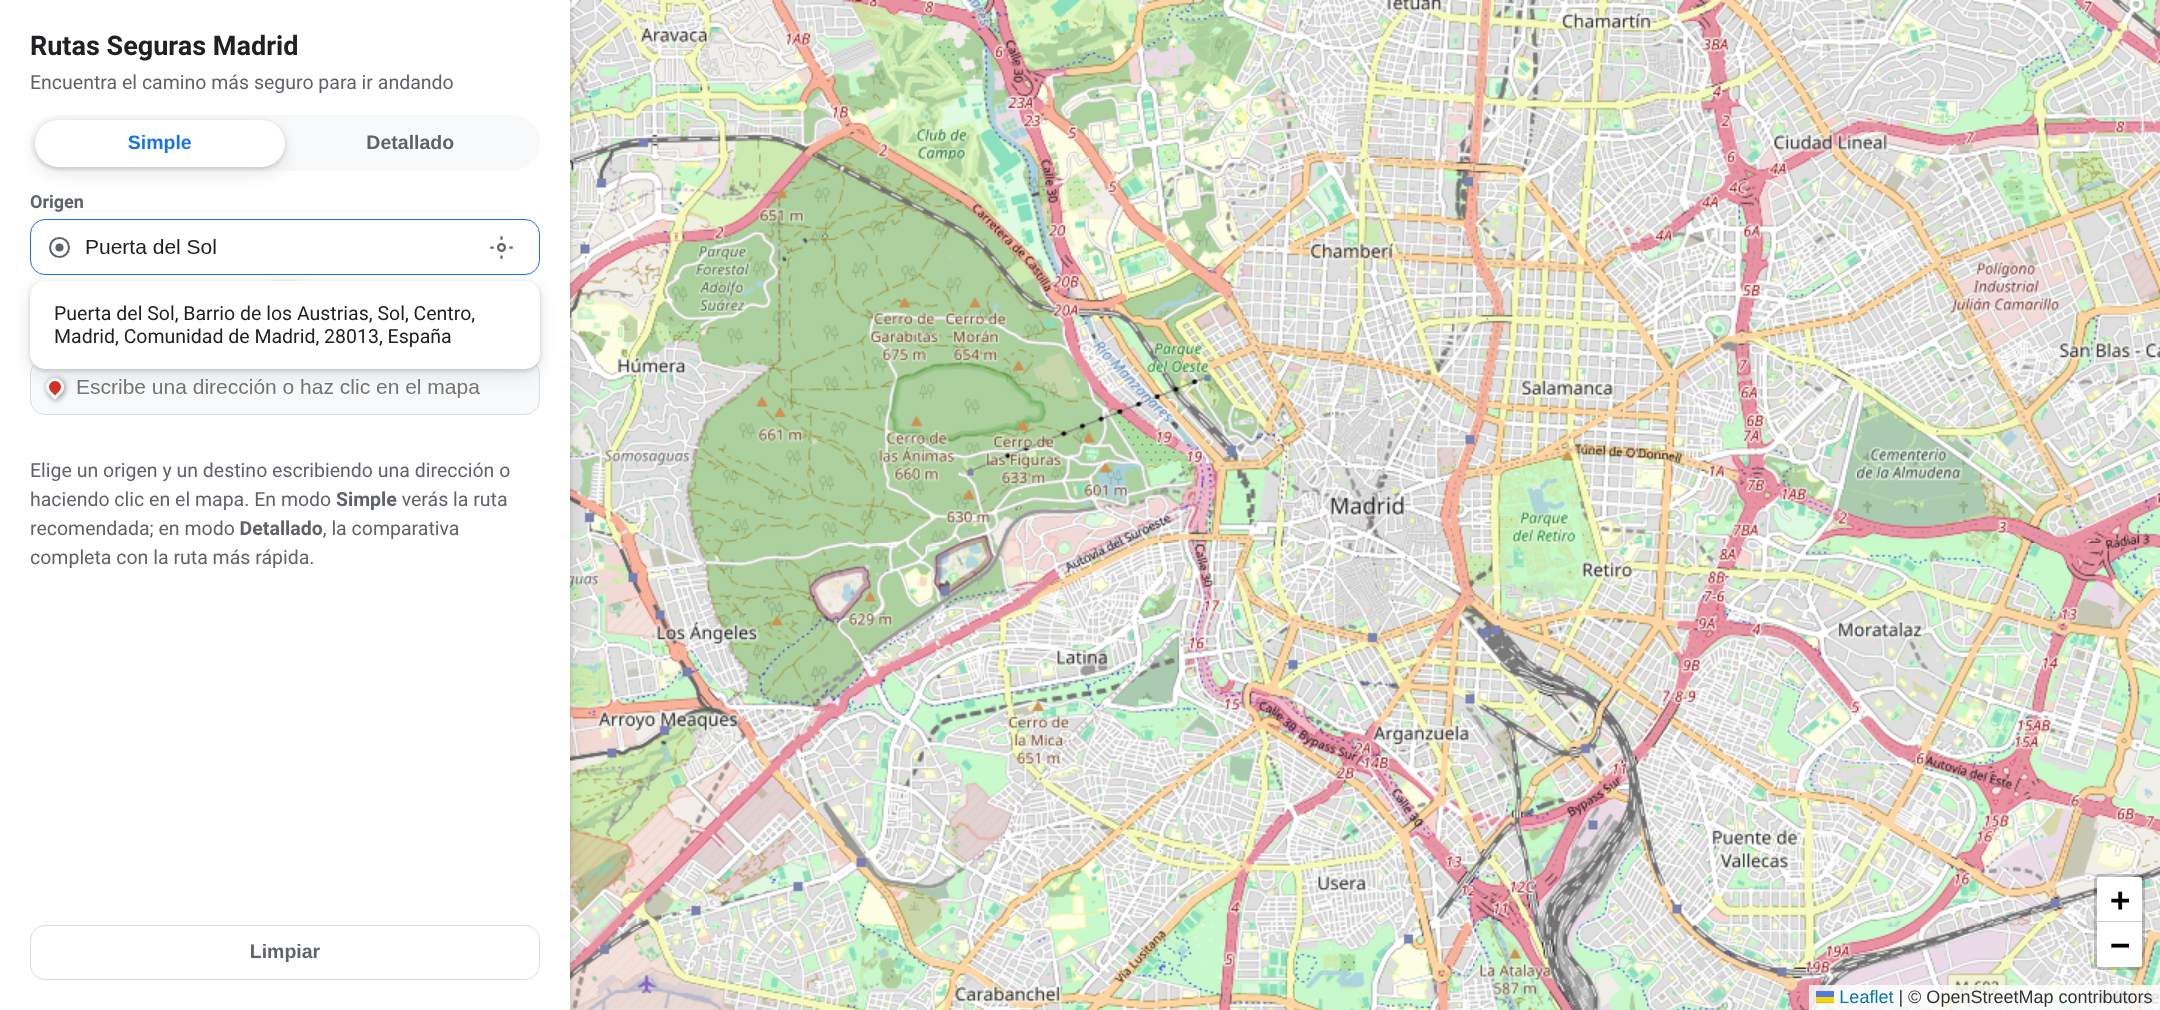
\includegraphics[width=\textwidth]{imagenes/visor_buscador.png}
\caption{Buscador de direcciones con autocompletado contra \texttt{/api/geocode}, mostrando las sugerencias para "Paseo de la Castellana 22".}
\label{fig:visor_buscador}
\end{figure}

Las Figuras~\ref{fig:visor_simple} y~\ref{fig:visor_detallado} muestran el prototipo en funcionamiento sobre el par Puerta del Sol -- Atocha, uno de los pares origen-destino que se retoman con más detalle en la evaluación del Capítulo~\ref{cap:pruebas}. En el modo simple (Figura~\ref{fig:visor_simple}) se aprecia la ruta recomendada, su distancia y duración, y la insignia cualitativa de seguridad (\textit{Segura} en este caso). En el modo detallado (Figura~\ref{fig:visor_detallado}) se superponen ambas rutas —discontinua en azul la rápida, continua en verde la segura— junto con la tabla comparativa de indicadores, cuyos valores coinciden con los recogidos más adelante en la Tabla~\ref{tab:resultados_rutas}.

\begin{figure}[h]
\centering
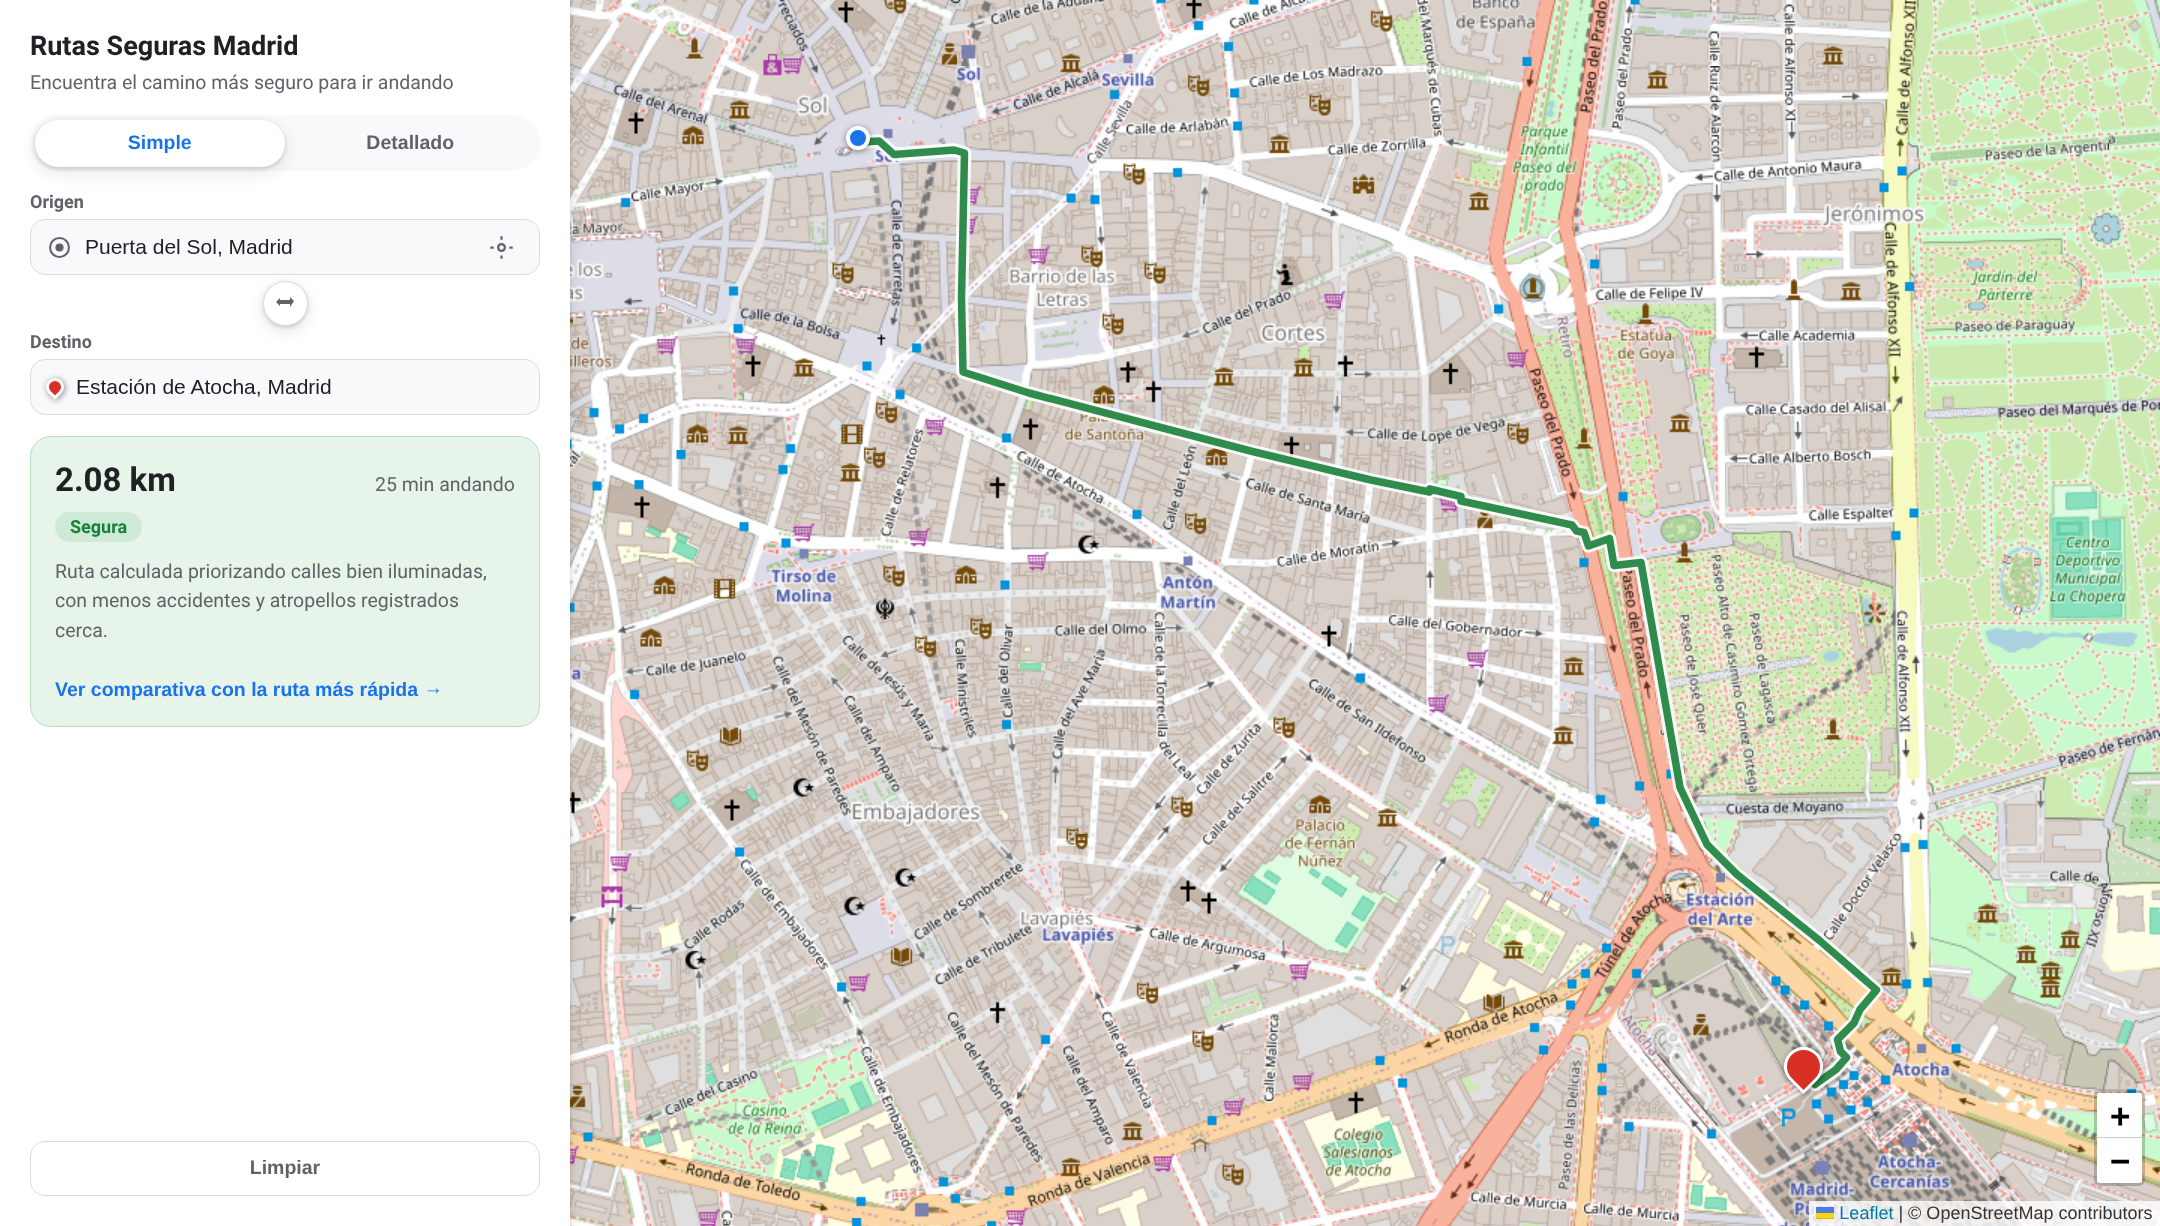
\includegraphics[width=\textwidth]{imagenes/visor_simple.png}
\caption{Visor web, modo simple, para el trayecto Puerta del Sol -- Atocha.}
\label{fig:visor_simple}
\end{figure}

\begin{figure}[h]
\centering
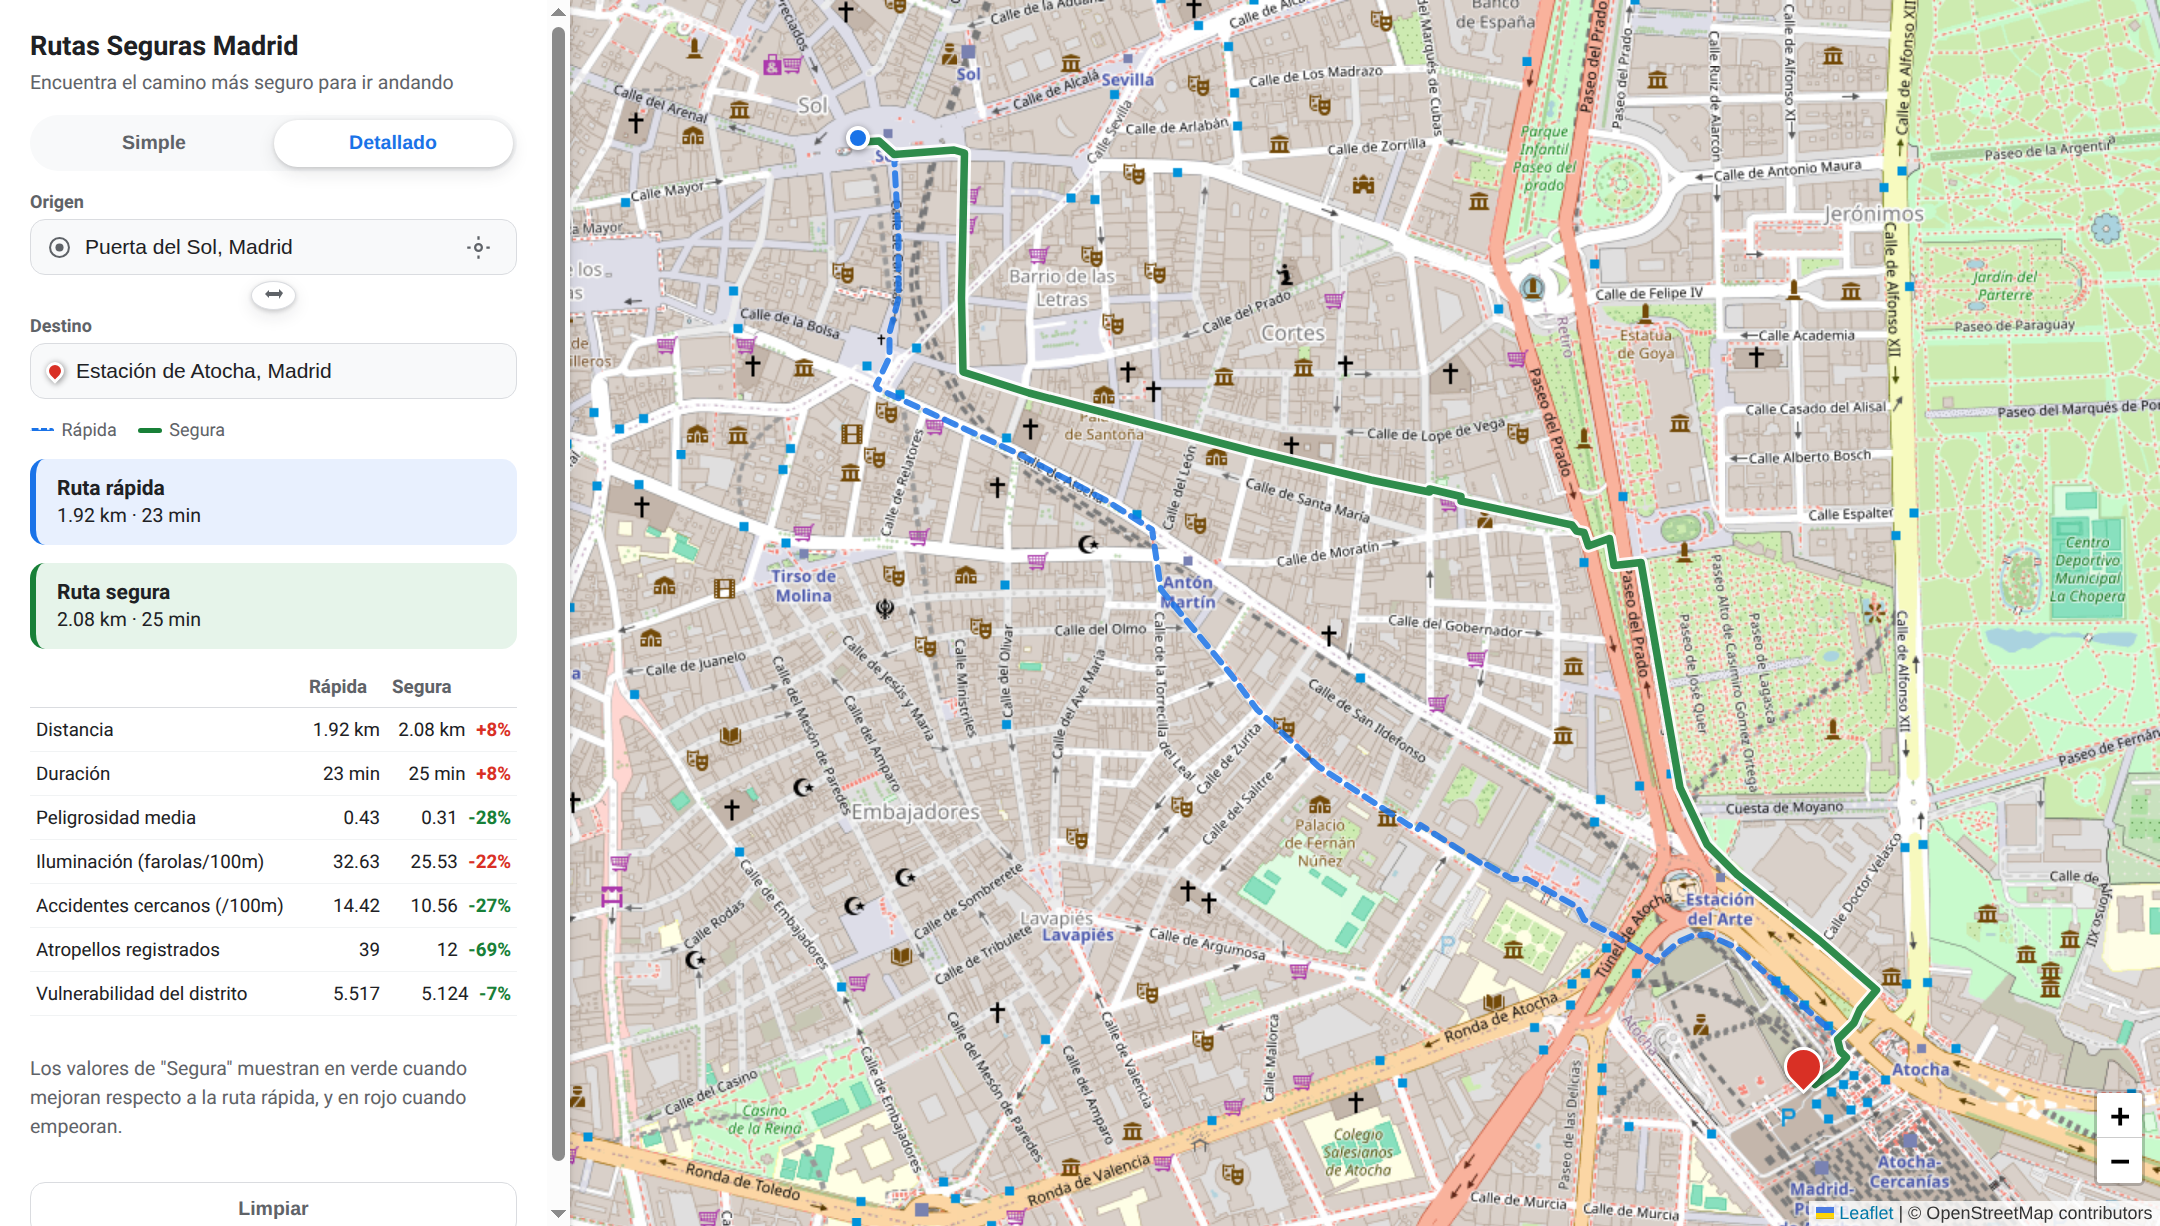
\includegraphics[width=\textwidth]{imagenes/visor_detallado.png}
\caption{Visor web, modo detallado, para el mismo trayecto: comparativa entre la ruta rápida y la ruta segura.}
\label{fig:visor_detallado}
\end{figure}
